\documentclass[12pt,letterpaper]{article}

% Librerías a utilizar
\usepackage[utf8]{inputenc}	% Codificación
\usepackage[spanish]{babel}	% Idioma
\usepackage{natbib}			% Bibliografía
\usepackage{graphicx}		% Imagenes
\usepackage{indentfirst}		% Sangría
\usepackage{amsmath, amsfonts, amssymb}	% Figuras matemáticas
\usepackage{url}    % URL
\usepackage{float}  % poscicionar imagenes


\usepackage[left=3cm,right=2cm,top=2cm,bottom=3cm]{geometry}

\setlength{\parindent}{2cm}	% Sangría en los párrafos
\renewcommand{\baselinestretch}{1.5}	% Interlineado

% Renombrar ciertos títulos del texto
\renewcommand\spanishcontentsname{Tabla de contenidos}
\renewcommand\spanishrefname{Bibliografía}

% Inicio del documento
\begin{document}

%%%%%%%%% PORTADA %%%%%%%%%

\newpage
\vspace*{-.5cm}
% Logo institucional
\begin{picture}(18,4)(0,30)
	\put(350,-20){
\includegraphics[scale=0.25]{./images/LogoUsach.pdf}}
\end{picture}

\sloppy
\thispagestyle{empty}
\vspace*{-1.6cm}

% Datos institucionales
\begin{center}
	{\bf \mbox{\large UNIVERSIDAD DE SANTIAGO DE CHILE}}\\
	{\bf \mbox{FACULTAD DE INGENIER\'IA}}\\
	{\bf \mbox{DEPARTAMENTO DE INGENIER\'IA INFORM\'ATICA}}\\
\end{center}

	\vspace{5cm}
	%Título del trabajo
	\begin{center}
	\Large
		\textbf{Laboratorio N 1}
	\end{center}

	% Datos personales
	\vspace*{6.25cm}
	\begin{flushright}
		\begin{tabular}[t]{l l}
			Integrantes: &Bastián Vera Palacios\\
			Curso: &Organización de Computadores\\
			Sección &0-L-3\\
			Profesor(a): &Leonel Medina Daza\\
			Ayudante : &Ricardo Álvarez Zambrano

		\end{tabular}
	\end{flushright}
	\begin{center}
		\vspace{1.5cm}
		% Fecha
		\Today
	\end{center}

\newpage
\tableofcontents
\thispagestyle{empty}

\newpage
\renewcommand{\thepage}{\arabic{page}}
\setcounter{page}{1}

% Capítulos agregados
\section{Introducción}

\subsection{Contexto}
\noindent La necesidad de buscar un medio de entretención ha sido parte de la sociedad desde tiempos remotos. Así mismo es donde bajo este contexto en persia, alrededor del siglo V, se dio la creación del juego Tic Tac Toe, Tres en Línea, Ceros y Cruces, entre otros nombres. Este juego fue difundido por los musulmanes y posteriormente llevado a europa por comerciantes italianos. El juego tuvo un rápido reconocimiento, aunque tuvo un periodo oscuro donde por una asociación de este con rituales paganos macabros, este estuvo prohibido para todos los cristianos de fe catolica. \citep{TicTacToe}

\noindent El juego consiste en una cuadrícula de 3x3 dentro de los cuales cada jugador debe colocar su símbolo una vez por turno y no debe ser sobre una casilla ya jugada. El ganador del juego es el jugador el cual logre realizar una línea recta o diagonal entre 3 de sus símbolos.

\subsection{Problema}

\noindent En este laboratorio se le solicitó a los estudiantes de ingeniería informática de la Universidad de Santiago de Chile realizar mediante una serie de algoritmos en lenguaje C, un programa que reciba un archivo de entrada con instrucciones en formato MIPS y que permita generar una partida del juego gato, es decir, poder entregar quién fue el ganador de la partida, especificar el caso en que exista un empate o que las instrucciones hayan generado una jugada invalida ,todo esto con el fin de poder medir las habilidades adquiridas durante el desarrollo de éste curso y a la vez entregar la cantidad de veces que se ha utilizado cada etapa del camino de datos.

\subsection{Motivación}
\noindent La compresión de un bajo nivel de abastracción se vuelve una ventaja comparativa al conocer cómo el software y hardware trabajan en conjunto y más especificamente, como este ultimo ejecuta las instrucciones de programa, ya que permite el desarrollo de programas más robustos, optimizados y que aprovechan al máximo el procesador.

\subsection{Objetivos}
\subsubsection{Objetivo general}
\noindent Simular el camino de datos de un procesador monociclo y determinar qué unidades funcionales del procesador son utilizadas en secuencias de instrucciones predefinida.
\subsubsection{Objetivos específicos}
\noindent Entender la importancia de las líneas de control en el camino de datos y el paso de las instrucciones a través de estas.

\subsection{Propuesta de solución}

\noindent A primera vista, se propone generar una estructura para definir el formato de una jugada. Posterior a esto se plantea manejar el tablero a través de un arreglo estático el cual maneje las posiciones del tablero. Una vez realizado lo anterior, se deberá realizar la lectura de las instrucciones y a partir de las distintas condiciones, ir insertando o eliminando jugadas, dependiendo del caso. Para finalizar se realizarán las comprobaciones finales en el tablero.

\subsection{Herramientas}
\noindent Dentro de las Herramientas para el desarrollo de este laboratorio se encuentran:

\begin{enumerate}
    \item Lenguaje de programación C con sus respectivos recursos, tales como punteros y memoria dinámica, entre otros.
    \item Librerías asociadas al lenguaje mencionado anteriormente, tales como \textit{stdio.h} y \textit{stdlib.h}.
\end{enumerate}

\subsection{Estructura del informe}
\noindent El presente escrito presenta a continuación conceptos que fueron la base principal en la que se desarro   lló la solución del problema, tales como punteros, memoria dinámica, entre otros, con el fin de exponer la investigación realizada, la descripción de la solución, el análisis de estos y las conclusiones.

\section{Marco teórico}

\subsection{Librerias}
\noindent Entre las herramientas utilizadas para el desarrollo de este laboratorio, se encuentran las librerías de:

\begin{itemize}
	\item stdio.h: Para la entrada, salida de datos y manejo de archivos.
    \item stdlib.h: Utilizada para el manejo de la memoria dinámica
	\item string.h: Utilizada para el manejo de concatenaciones de caracteres.
\end{itemize}

\subsection{MIPS (Procesador)}
\noindent Con el nombre de MIPS, se le conoce a la familia de microprocesadores de arquitectura RISC desarrollados por MIPS Technologies, diseñado para optimizar segmentación en unidades de control y facilitar la generación automática de código maquina por parte de los compiladores.

\subsection{Registro}
\noindent Un registro corresponde al hardware que forma parte del procesador y puede contener una determinada cantidad de bits. Estos ofreces un nivel de memoria más rapido y acotado que la memoria principal, son empleados para controlar las instrucciones de ejecución, manejar el direccionamiento de memoria y proporcionar capacidad aritmética.

\subsection{Punteros}
\noindent Los punteros son elementos bastante utilizados durante el desarrollo del código debido a que permiten trabajar directamente a las direcciones de memoria de las estructuras de datos que tenemos. Se utilizan tanto como para lectura del archivo como para poder almacenar cada elemento de la instrucción en su estructura correspondiente.

\subsection{Lectura y escritura de archivos}
\noindent Para poder realizar la lectura de archivos anexos a los ingresados manualmente por terminal en nuestro código se utilizan funciones específicas llamadas por la librería stdio.h las cuales nos facilitan el acceso a éstos.

\subsection{Memoria dinámica}
\noindent Para un óptimo avance en este código se utilizó memoria dinámica durante la inicialización de las estructuras con el fin de que se pueda trabajar con los valores leídos en el archivo de manera más eficiente. Para esto se utilizó la función malloc() para poder asignar el espacio propio de cada instrucción y la función free() para ir liberando la memoria una vez que ésta ya ha sido utilizada.

\subsection{Estructuras}
\noindent Las estructuras son un tipo de dato utilizado para poder agrupar distintos tipos de información y manejar datos que sería muy complicado de realizar de manera más primitiva. En el desarrollo de este código se utilizan para la implementación de los nodos del árbol ya que así se puede acceder de manera inmediata a la información contenida en éstos.

\section{Desarollo}

\noindent Para el desarrollo de este laboratorio lo primero que se realiza es una estructura la cual almacene de manera eficiente para un posterior trabajo la instrucción a leer. Para esto se crea la estructura \textit{Move} la cual posee 4 punteros de tipo char, los cuales almacenarán específicamente la instrucción, 2 registros, y un valor numérico (el cual solo se emplea para los registros \textit{addi} y \textit{subi}).

\begin{figure}[H]
	\centering
	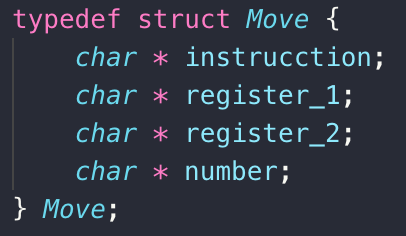
\includegraphics[scale=1]{images/estructura.png}
	\caption{Archivo de salida del camino de datos.}
	\label{fig:estructura}
\end{figure}

\noindent Posterior a esto se realiza la lectura de cada línea del archivo de entrada, donde se revisa la primera palabra de la línea; si esta es una instrucción, dependiendo de su tipo, se realiza una lectura de los registro y datos asociados a este, para así asociarlo a una estructura la cual será almacenada posterior a este proceso en un arreglo que contendrá todas las estructuras.

\noindent Una vez que todas las instrucciones se encuentren almacenadas de manera correcta en el arreglo de estructuras, se prosigue con la evaluación de cada una de estas y su respectiva función y a la declaración de un tablero, el cual consiste en un arreglo de caracteres con un largo de 9, el cual representará el tablero matricial.

\noindent En primera instancia se revisan las primeras dos instrucciones y las define como los jugadores (jugador X y jugador O), ambas entregadas por una instrucción de tipo \textit{addi}. En la siguiente línea se verifica que se pida el almacenamiento para las jugadas a insertar. Posterior a estas 3 revisiones principales, se recorre el arreglo leyendo el tipo de instrucción que posee cada una de las instrucciones y según ésta, define qué acción realizará. Antes de realizar la acción, se le realiza la consulta al tablero si la jugada, ya sea insertar o eliminar un símbolo, exista y que a la vez, esta sea propia del jugador que quiere realizar la acción.En el caso que se realice una jugada no válida, tal como la inserción en alguna casilla no existente o la sobrescritura respecto una jugada del otro jugador, el programa entrega un mensaje que la partida está incompleta y procede al cierre de este.

 \noindent Al final de la lectura de todas las instrucciones del arreglo, se realiza una comprobación respecto a si hay un ganador (indicando el nombre de este en caso de existir) o si se genera un empate. Para realizar el cálculo de cuántas veces pasa cada instrucción por cada etapa en el camino de datos, se realizan sumas de valor 1 por cada etapa que realiza de manera constante cada instrucción, es decir, se asume que si es una instrucción de tipo \textit{addi} o \textit{subi}, estas pasarán por las 5 etapas del camino de datos, en cambio, una instrucción de tipo \textit{sw} solamente utiliza 4 etapas del camino de datos (se excluye Mem). A modo de finalización, el programa entrega dos documentos, uno llamado \textit{resultado.txt}, el cual posee la respuesta del ganador de la partida en caso de existir y el tablero con las jugadas realizadas, y un documento llamado \textit{Etapas.txt}, el cual entrega la cantidad de veces que cada instrucción pasa por cada etapa del camino de datos del procesador monociclo.

\section{Experimentos a realizar}


\subsection{Resultados obtenidos}
\noindent A continuación se presentan los archivos de salida resultantes posterior a un caso de prueba.
\begin{figure}[H]
	\centering
	\includegraphics[scale=0.5]{images/compilacion.png}
	\caption{Ejemplo Salida al compilar el codigo.}
	\label{fig:ej1}
\end{figure}

\begin{figure}[H]
	\centering
	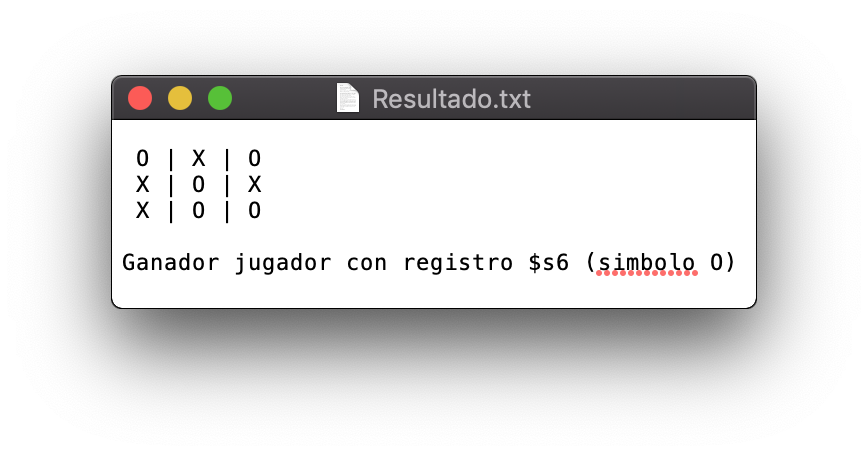
\includegraphics[scale=0.5]{images/resultado.png}
	\caption{Ejemplo de Salida del resultado del juego.}
	\label{fig:ej2}
\end{figure}

\begin{figure}[H]
	\centering
	\includegraphics[scale=0.5]{images/Etapas.png}
	\caption{Archivo de salida del camino de datos.}
	\label{fig:ej3}
\end{figure}


\subsection{Análisis de resultados}

\noindent Se ha logrado que el programa sea capaz de leer las instrucciones y las líneas de control que se presentan en un archivo de texto plano, distinguiendo en este los comentarios y valores inválidos dentro de una jugada, para luego simular su ejecución completando el tablero de manera óptima, en caso que las instrucciones se encuentren insertadas de manera correcta. El programa logra identificar de manera adecuada cuando una jugada corresponde a la victoria de un jugador en particular, un empate o un error de instrucción, el cuál entrega un mensaje de "incompleto".

\section{Conclusiones}

\noindent Gracias a el desarrollo de este laboratorio se puede apreciar de mejor manera el manejo de los conocimientos ya adquiridos durante el desarrollo de las clases, ya que en cada uno de éstos, se profundizaron temas que ahora nos facilitan la compresión del camino de datos y como este es realizado por los distintos tipos de instrucciones que se pueden realizar. Referente a los algoritmos utilizados estos trabajan de manera correcta, gracias a una correcta implementación de la estructura \textit{Move}, el cual facilitó el manejo independiente de cada elemento agrupado en este. Respecto a objetivos planteados en este laboratorio, el programa funciona de manera correcta entregando los valores del camino de datos empleados y el resultado de la partida.


\clearpage
\addcontentsline{toc}{section}{Bibliografía}
\bibliographystyle{apalike}
\bibliography{bibliografia}


\end{document}
